% This is "sig-alternate.tex" V2.1 April 2013
% This file should be compiled with V2.5 of "sig-alternate.cls" May 2012
%
% This example file demonstrates the use of the 'sig-alternate.cls'
% V2.5 LaTeX2e document class file. It is for those submitting
% articles to ACM Conference Proceedings WHO DO NOT WISH TO
% STRICTLY ADHERE TO THE SIGS (PUBS-BOARD-ENDORSED) STYLE.
% The 'sig-alternate.cls' file will produce a similar-looking,
% albeit, 'tighter' paper resulting in, invariably, fewer pages.
%
% ----------------------------------------------------------------------------------------------------------------
% This .tex file (and associated .cls V2.5) produces:
%       1) The Permission Statement
%       2) The Conference (location) Info information
%       3) The Copyright Line with ACM data
%       4) NO page numbers
%
% as against the acm_proc_article-sp.cls file which
% DOES NOT produce 1) thru' 3) above.
%
% Using 'sig-alternate.cls' you have control, however, from within
% the source .tex file, over both the CopyrightYear
% (defaulted to 200X) and the ACM Copyright Data
% (defaulted to X-XXXXX-XX-X/XX/XX).
% e.g.
% \CopyrightYear{2007} will cause 2007 to appear in the copyright line.
% \crdata{0-12345-67-8/90/12} will cause 0-12345-67-8/90/12 to appear in the copyright line.
%
% ---------------------------------------------------------------------------------------------------------------
% This .tex source is an example which *does* use
% the .bib file (from which the .bbl file % is produced).
% REMEMBER HOWEVER: After having produced the .bbl file,
% and prior to final submission, you *NEED* to 'insert'
% your .bbl file into your source .tex file so as to provide
% ONE 'self-contained' source file.
%
% ================= IF YOU HAVE QUESTIONS =======================
% Questions regarding the SIGS styles, SIGS policies and
% procedures, Conferences etc. should be sent to
% Adrienne Griscti (griscti@acm.org)
%
% Technical questions _only_ to
% Gerald Murray (murray@hq.acm.org)
% ===============================================================
%
% For tracking purposes - this is V2.0 - May 2012

\documentclass{sig-alternate-05-2015}

\usepackage{tikz}
\usetikzlibrary{arrows,positioning,automata}
\usepackage[noend]{algpseudocode}
\usepackage{algorithm}
\usepackage{enumitem, kantlipsum}
\usepackage{adjustbox}
\usepackage{multirow}

% Use the postscript times font!
\usepackage{times}

\usepackage{mathtools}
\usepackage{amssymb}

\begin{document}

% Copyright
\setcopyright{acmcopyright}
%\setcopyright{acmlicensed}
%\setcopyright{rightsretained}
%\setcopyright{usgov}
%\setcopyright{usgovmixed}
%\setcopyright{cagov}
%\setcopyright{cagovmixed}


% DOI
\doi{10.475/123_4}

% ISBN
\isbn{123-4567-24-567/08/06}

%Conference
\conferenceinfo{PLDI '13}{June 16--19, 2013, Seattle, WA, USA}

\acmPrice{\$15.00}

%
% --- Author Metadata here ---
\conferenceinfo{WOODSTOCK}{'97 El Paso, Texas USA}
%\CopyrightYear{2007} % Allows default copyright year (20XX) to be over-ridden - IF NEED BE.
%\crdata{0-12345-67-8/90/01}  % Allows default copyright data (0-89791-88-6/97/05) to be over-ridden - IF NEED BE.
% --- End of Author Metadata ---

\title{``It Was Not Your Fault'' -- Emotional Awareness Improves Collaborative
Robots}
% \subtitle{[Extended Abstract]
%
% You need the command \numberofauthors to handle the 'placement
% and alignment' of the authors beneath the title.
%
% For aesthetic reasons, we recommend 'three authors at a time'
% i.e. three 'name/affiliation blocks' be placed beneath the title.
%
% NOTE: You are NOT restricted in how many 'rows' of
% "name/affiliations" may appear. We just ask that you restrict
% the number of 'columns' to three.
%
% Because of the available 'opening page real-estate'
% we ask you to refrain from putting more than six authors
% (two rows with three columns) beneath the article title.
% More than six makes the first-page appear very cluttered indeed.
%
% Use the \alignauthor commands to handle the names
% and affiliations for an 'aesthetic maximum' of six authors.
% Add names, affiliations, addresses for
% the seventh etc. author(s) as the argument for the
% \additionalauthors command.
% These 'additional authors' will be output/set for you
% without further effort on your part as the last section in
% the body of your article BEFORE References or any Appendices.

\numberofauthors{4} %  in this sample file, there are a *total*
% of EIGHT authors. SIX appear on the 'first-page' (for formatting
% reasons) and the remaining two appear in the \additionalauthors section.
%
\author{
% You can go ahead and credit any number of authors here,
% e.g. one 'row of three' or two rows (consisting of one row of three
% and a second row of one, two or three).
%
% The command \alignauthor (no curly braces needed) should
% precede each author name, affiliation/snail-mail address and
% e-mail address. Additionally, tag each line of
% affiliation/address with \affaddr, and tag the
% e-mail address with \email.
%
% 1st. author
\alignauthor
Mahni Shayganfar \\
       \affaddr{Worcester Polytechnic Institute}\\
       \affaddr{100 Institute Road}\\
       \affaddr{Worcester, MA 01609}\\
       \email{mshayganfar@wpi.edu}
% 2nd. author
\alignauthor
Charles Rich \\
       \affaddr{Worcester Polytechnic Institute}\\
       \affaddr{100 Institute Road}\\
       \affaddr{Worcester, MA 01609}\\
       \email{rich@wpi.edu}
\and
% 3rd. author
\alignauthor 
Candace L. Sidner\\
       \affaddr{Worcester Polytechnic Institute}\\
       \affaddr{100 Institute Road}\\
       \affaddr{Worcester, MA 01609}\\
       \email{sidner@wpi.edu}
% 4th. author
\alignauthor 
Benjamin L. Hyl\'ak\\
       \affaddr{Worcester Polytechnic Institute}\\
       \affaddr{100 Institute Road}\\
       \affaddr{Worcester, MA 01609}\\
       \email{blhylak@wpi.edu}
}
% There's nothing stopping you putting the seventh, eighth, etc.
% author on the opening page (as the 'third row') but we ask,
% for aesthetic reasons that you place these 'additional authors'
% in the \additional authors block, viz.

% \additionalauthors{Additional authors: John Smith (The Th{\o}rv{\"a}ld Group,
% email: {\texttt{jsmith@affiliation.org}}) and Julius P.~Kumquat
% (The Kumquat Consortium, email: {\texttt{jpkumquat@consortium.net}}).}
% \date{30 July 1999}

% Just remember to make sure that the TOTAL number of authors
% is the number that will appear on the first page PLUS the
% number that will appear in the \additionalauthors section.

\maketitle
\begin{abstract}
We have conducted a user study to investigate the importance of emotional
awareness and the underlying affect-driven processes during a human-robot
collaboration. The goal of this user study was twofold: (1) Investigating the 
overall functionality of the mechanisms and the underlying algorithms in our
architecture, (2) Evaluating human's willingness and assessment of collaboration
with an emotion-aware and an emotion-ignorant robot. We designed a simple table
top game to simulate the collaborative environment in which a participant and
the robot were ``installing'' a solar panel together. The result of our user
study shows a significant difference between humans' preference of working with
an emotion-aware robot during collaboration.
\end{abstract}


%
% The code below should be generated by the tool at
% http://dl.acm.org/ccs.cfm
% Please copy and paste the code instead of the example below. 
%
\begin{CCSXML}
<ccs2012>
 <concept>
  <concept_id>10010520.10010553.10010562</concept_id>
  <concept_desc>Computer systems organization~Embedded systems</concept_desc>
  <concept_significance>500</concept_significance>
 </concept>
 <concept>
  <concept_id>10010520.10010575.10010755</concept_id>
  <concept_desc>Computer systems organization~Redundancy</concept_desc>
  <concept_significance>300</concept_significance>
 </concept>
 <concept>
  <concept_id>10010520.10010553.10010554</concept_id>
  <concept_desc>Computer systems organization~Robotics</concept_desc>
  <concept_significance>100</concept_significance>
 </concept>
 <concept>
  <concept_id>10003033.10003083.10003095</concept_id>
  <concept_desc>Networks~Network reliability</concept_desc>
  <concept_significance>100</concept_significance>
 </concept>
</ccs2012>  
\end{CCSXML}

\ccsdesc[500]{Computer systems organization~Embedded systems}
\ccsdesc[300]{Computer systems organization~Redundancy}
\ccsdesc{Computer systems organization~Robotics}
\ccsdesc[100]{Networks~Network reliability}


%
% End generated code
%

%
%  Use this command to print the description
%
\printccsdesc

% We no longer use \terms command
%\terms{Theory}

\keywords{Human-Robot Collaboration, Affect-Driven Processes, Emotion-Awareness}

\section{Introduction}
The idea of robots or other intelligent agents living in a human environment has
been a persistent dream from science fiction books to artificial intelligence
and robotic laboratories. Collaborative robots are expected to become an
integral part of humans' environment to accomplish their industrial and
household tasks. In these environments, humans will be involved in robots'
operations and decision-making processes. The involvement of humans influences
the efficiency of robots' interaction and performance, and makes the robots
sensitive to humans' cognitive abilities and internal states.

We believe that collaborative robots need to take into account humans' internal
states while making decisions during collaboration. Humans express emotions to
reveal their internal states in social contexts including collaboration
\cite{breazeal:sociable-interactive-robots}. Due to the existence of such
expressions robot's emotional-awareness can improve the quality of collaboration
in terms of humans' perception of performance and preferences. Hence,
collaborative robots require to include affect-driven mechanisms in their
decision making processes to be able to interpret and generate appropriate
responses and behaviors. Our aim in this work was to study the importance of
emotional awareness and the underlying affect-driven processes in human-robot
collaboration. We examined how emotional-awareness impacts different aspects of
humans' preferences by comparing the results from our participants collaborating
with an emotion-aware and an emotion-ignorant robot.

This work is implemented as part of a larger effort to assess affect-driven
collaborative robots which are capable of generating and recognizing emotions in
order to be better collaborators. This work is based on the development of
\textit{Affective Motivational Collaboration Theory} which is built on the
foundations of the \textit{SharedPlans} theory of collaboration
\cite{grosz:plans-discourse} and the \textit{cognitive appraisal} theory of
emotions \cite{gratch:domain-independent}.

\section{Related Work}

There are many research areas, including robotics and autonomo-us agents, that
employ the structure and/or functions of emotions in their work with a variety
of motivations behind modeling emotions
\cite{wehrle:motivations-modeling-emotion}. In
\cite{breazeal:sociable-interactive-robots} authros surveyed some of the
principle research in social robotics and its applications in Human-Robot
Interaciton. We can see the application of emotion theories in designing robots
capable of learning from humans \cite{breazeal:expressive-behavior}, robots
capable of expressing emotions \cite{cameron:expression-hri}
\cite{shayganfar:methodology} and social behaviors
\cite{paiva:emotion-modeling}, as well as robots which can convey certain types
of emotion products, e.g., empathy \cite{leite:empathy-hri}. There are also
several works in which researchers have explored the human's affective state as
a mechanism to adapt the robot's behaviors during the interaction
\cite{breazeal:sociable-robot} \cite{liu:affect-robot-behavior}.

\begin{figure*}[tbh]
  \centering
  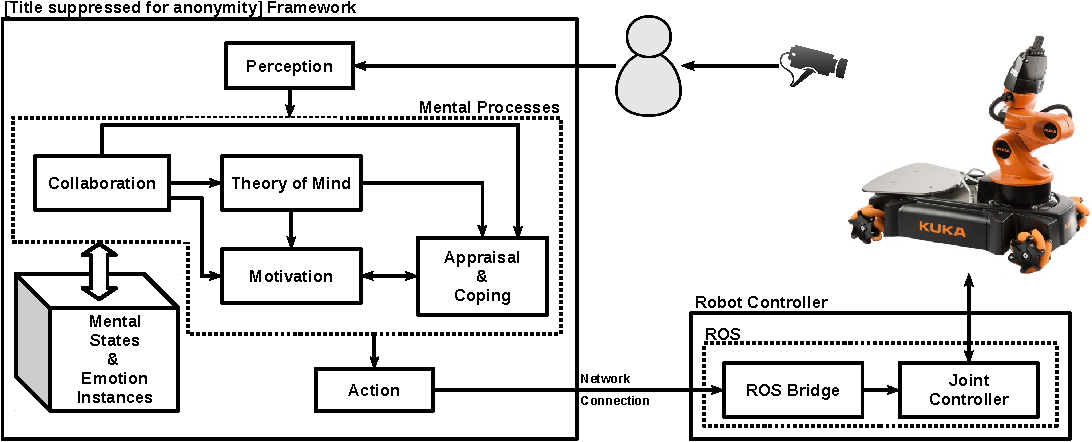
\includegraphics[width=\textwidth]{figure/framework-croped.pdf}
  \caption{{\fontsize{9}{9}\selectfont Computational framework based on
  [title suppressed for anonymity] theory (arrows indicate primary influences
  between mechanisms and data flow).}}
  \vspace*{-5mm}
  \label{fig:framework}
\end{figure*}

Many of the computational models of emotions and their applications are derived
from appraisal theories of emotion making appraisal as the central process in
their architectures \cite{adam:bdi-emotional-companion}
\cite{marinier:behavior-emotion} \cite{marsella:ema-process-model}
\cite{si:modeling-appraisal-tom-journal}. Appraisal is usually modeled as the
cause of emotion being derived via simple rules on a set of appraisal variables.
In robotics, appraisal theory has been used to establish and maintain a better
interaction between a robot and a human \cite{castro:autonomous-robot-fear}
\cite{kim:model-hri-appraisal} \cite{pontier:women-robot-men}
\cite{vogiatzis:robot-museum}. There are other models of emotions that have been
also used in robotics and human-robot interaction \cite{klug:emotion-based-hri}
\cite{lim:mei-motherese-ei} \cite{zhang:service-robot-dimensional}.

There are also other examples that researchers focus on the applications of
emotions in human-robot collaboration. For instance, in
\cite{guha:emotion-feedback} researchers use robot's emotional expression as a
feedback to the human to improve the quality of collaboraiton. In
\cite{looije:affective-collaboration-safety} authors introduce some theoretical
concepts that affective collaborative robots can enhance joint human-robot
performance by adapting the robot's role and interaction to the human's
affective state. This work does not provide any details of implementation and
how these theoretical concepts can lead to a better human-robot collaboration.
However, little effort has been put on development of functions of emotions and
their applications in decision making and emotional-awareness processes of
collaborative robots.

\section{Implementation}
The implementation of this user-study included two separated parts. The first
part incorporated the [Title Suppressed For Anony-mity] Framework consisting of
all Mental Processes (see left-side of Figure \ref{fig:framework}) briefly
described in Section \ref{sec:theory}. The second part was implemented to
recieve action commands from the framework and forwarding them to the robot to
control joints and actuators (see right-side of Figure \ref{fig:framework}).

\subsection{[Title Suppressed For Anonymity] Framework}
\label{sec:theory}
This framework is built based on [Title Suppressed For Anonym-ity] Theory which
deals with the interpretation and prediction of observable behaviors in a dyadic
collaboration \cite{shayganfar:theory-overview}. The theory focuses on the
processes regulated by emotional states \cite{shayganfar:goal-management}. The
observable behaviors represent the outcome of reactive and deliberative
processes related to the interpretation of the self's relationship to the
environment. [Title Suppressed For Anonymity] Theory aims to explain both rapid
emotional reactions to events as well as slower, more deliberative responses.
The reactive and deliberative processes are triggered by two types of events:
\textit{external} events, such as the other's \textit{utterances} and
\textit{primitive actions}, and \textit{internal} events, comprising changes in
the self's mental states, such as belief formation and emotional changes. The
theory explains how emotions regulate the underlying processes when these events
occur. It also elucidates the role of \textit{motives} as goal-driven
emotion-regulated constructs with which a robot can form new intentions to cope
with events.

The framework includes the mechanisms depicted as mental processes in Figure
\ref{fig:framework} along with the mental states. The mental
states shown in Figure \ref{fig:framework} comprise the knowledge base required
for all the mechanisms in the overall model. These \textit{mental states}
include self's (robot's) beliefs, intentions, motives, goals and emotion
instances as well as the anticipated mental states of the other (human). The
details about all these metal states are beyond the scope of this paper. 

Each mechanism includes one or more processes in our architecture. For instance,
the \textit{Collaboration} mechanism includes processes such as \textit{Focus
Shifting} and \textit{Constraint Management}, while the \textit{Appraisal}
mechanism includes processes to compute the values for individual appraisal
variables \cite{shayganfar:emotional-awareness}
\cite{shayganfar:appraisal-short}. The \textit{Collaboration} mechanism
maintains constraints on actions, including task states and the ordering of
tasks, and provides processes to update and monitor the shared plan. In this
user-study, the \textit{Collaboration} mechanism uses a hierarchy of goals
associated with tasks in a the Hierarchical Task Network (HTN) structure
depicted in Figure \ref{fig:collaboration_structure}. The \textit{Appraisal}
mechanism is responsible for evaluating changes in the self's mental states, the
anticipated mental states of the other, and the state of the collaboration
environment. The \textit{Coping} mechanism provides the self with different
coping strategies associated with changes in the self's mental states with
respect to the state of the collaboration. The \textit{Motivation} mechanism
operates whenever the self a) requires a new motive to overcome an internal
impasse in an ongoing task, or b) wants to provide an external motive to the
other (i.e. human) when the other faces a problem in a task. The \textit{Theory
of Mind} mechanism infers a model of the other's anticipated mental state. The
self progressively updates this model during the collaboration.

\begin{figure*}[tbh]
  \centering
  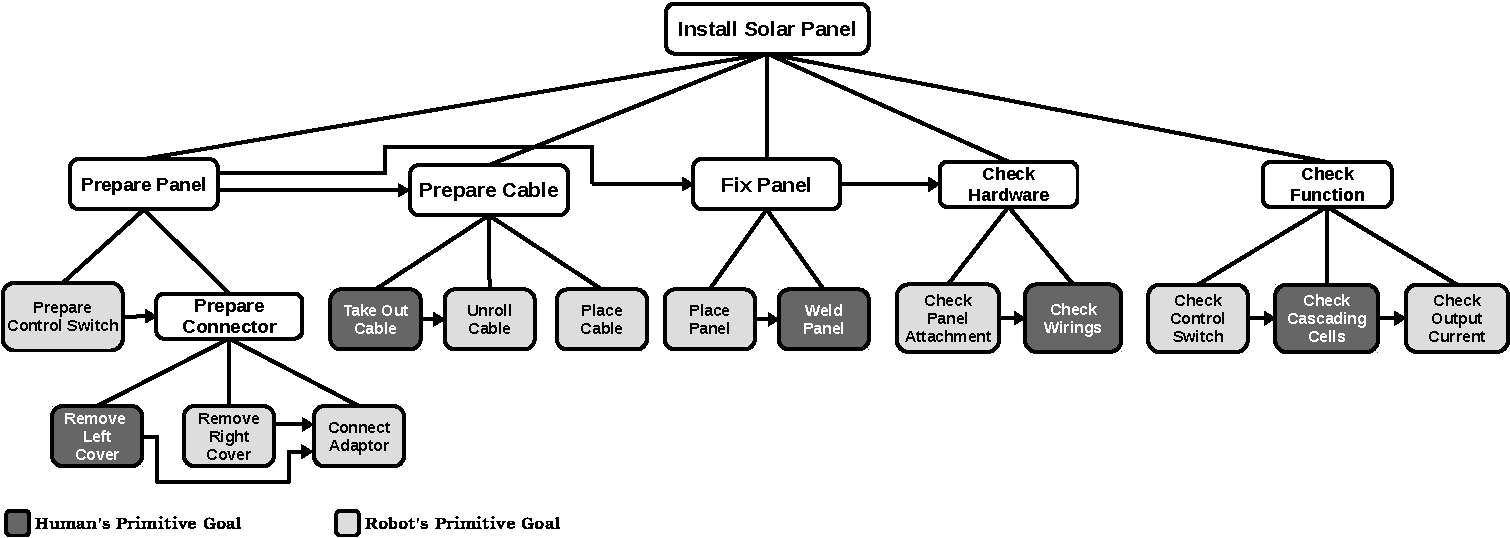
\includegraphics[width=1\textwidth]{figure/collaborationStructure.pdf}
  \caption{{\fontsize{9}{9}\selectfont Collaboration structure used as the
  task model.}}
  \vspace*{-5mm}
  \label{fig:collaboration_structure}
\end{figure*}

\subsection{Robot Controller}
The robot controller is comprised of two major components: ROS-bridge and joint
controller (see Figure \ref{fig:framework}).
Ros-bridge\footnote{http://wiki.ros.org/rosbridge\_suite} provides an API to ROS
functionality for non-ROS programs which enables us to send action commands from
our framework (implemented in JAVA) to the robot's joint controller. The joint
controller receives action commands and translates them into actual joint and
actuator commands and sends them to the robot.

\section{Experimental Scenario}

Our scenario was based on a table top turn-taking game that we designed to
simulate installing a solar panel. Participants had to collaborate one-on-one
with our robot to complete all the given tasks required to install the solar
panel. All the tasks were simple picking up and placing collaborators' available
pegs on predefined spots on the board (see Figure \ref{fig:game_board}). Each
pick-and-place was associated with the robot's or the participant's task. The
robot and the participants had their own unique primitive tasks that they had to
accomplish in their own turn. The final goal of installing a solar panel
required the robot and the participants to accomplish their own individual
tasks. Failure of any task could create an impasse during the collaboration.

\subsection{The Robot}

We conducted our experiment based on a KUKA Youbot (see Figure
\ref{fig:environment}). The robot was stationary on top of a desk and was able
to pick up and place avaiable pegs corresponding to the robot's task. The robot
was operated based on Robot Operating System (ROS) and was receiving commands
through the ROS-bridge from our [Title Suppressed For Anonymity] framework (see
Figure \ref{fig:framework}).

\subsection{Interaction Paradigms}
\label{sec-interaction-paradigms}
The robot interacted via a) speech, b) the corresponding utterance on the
screen, c) negative, positive and neutral expression of emotion through an
emoticon on the screen. The robot used neutral expression in case of the
emotion-ignorance. The interaction was controlled autonomously by the AMC
framework in case of the emotion-awareness, and Disco in case of the
emotion-ignorance (see Section XYZ). The reasoning about which task should be
done and controlling the robot was entirely autonomous. Only the perception of
the task failure or achievement by the robot or by the participant was done by a
wizard monitoring the collabortion outside of the test area. The interaction was
structured based on the exact same goals in an HTN for both conditions. The
robot was using the same utterances in both conditions. In emotion-aware
condition only if the participant was expressing a negative emotion in case of a
failure the robot was using a different utterance in compare to the
participant's positive or neutral expression of emotion; i.e., the robot's
utterances were identical in emotion-aware and emotion-ignorance cases if in the
latter the participant reported (expressed) a positive or a neutral emotion. At
the beginning of each collaboration the robot asked each participant to achieve
the overall shared goal, i.e., ``installing the solar panel''. Then, before
achieving a new goal, the robot informed the participant about the higher level
nonprimitive goal of which the primitives were going to be achieved. The same
procedure was used by the robot if there was a decision for switching to another
nonprimitive due to the failure of the task achieving the current goal. For
example, \ldots (see Figure \ref{fig:collaboration_structure}). After achieving
a new primitive goal, the robot either informed the human keeping the ground for
the next goal to achieve, or informed and passed the ground to the human to
execute the next task with repoect to the human's goal. In case of the human's
turn, the robot waited for the human to do a task, then the wizard let the robot
know whether the human's goal was achieved or not. Afterwards the robot was
making a decision about which goal to pursue and was informing human
accordingly. The same entire procedure was applied to both conditions.

\begin{figure}[tbh]
  \centering
  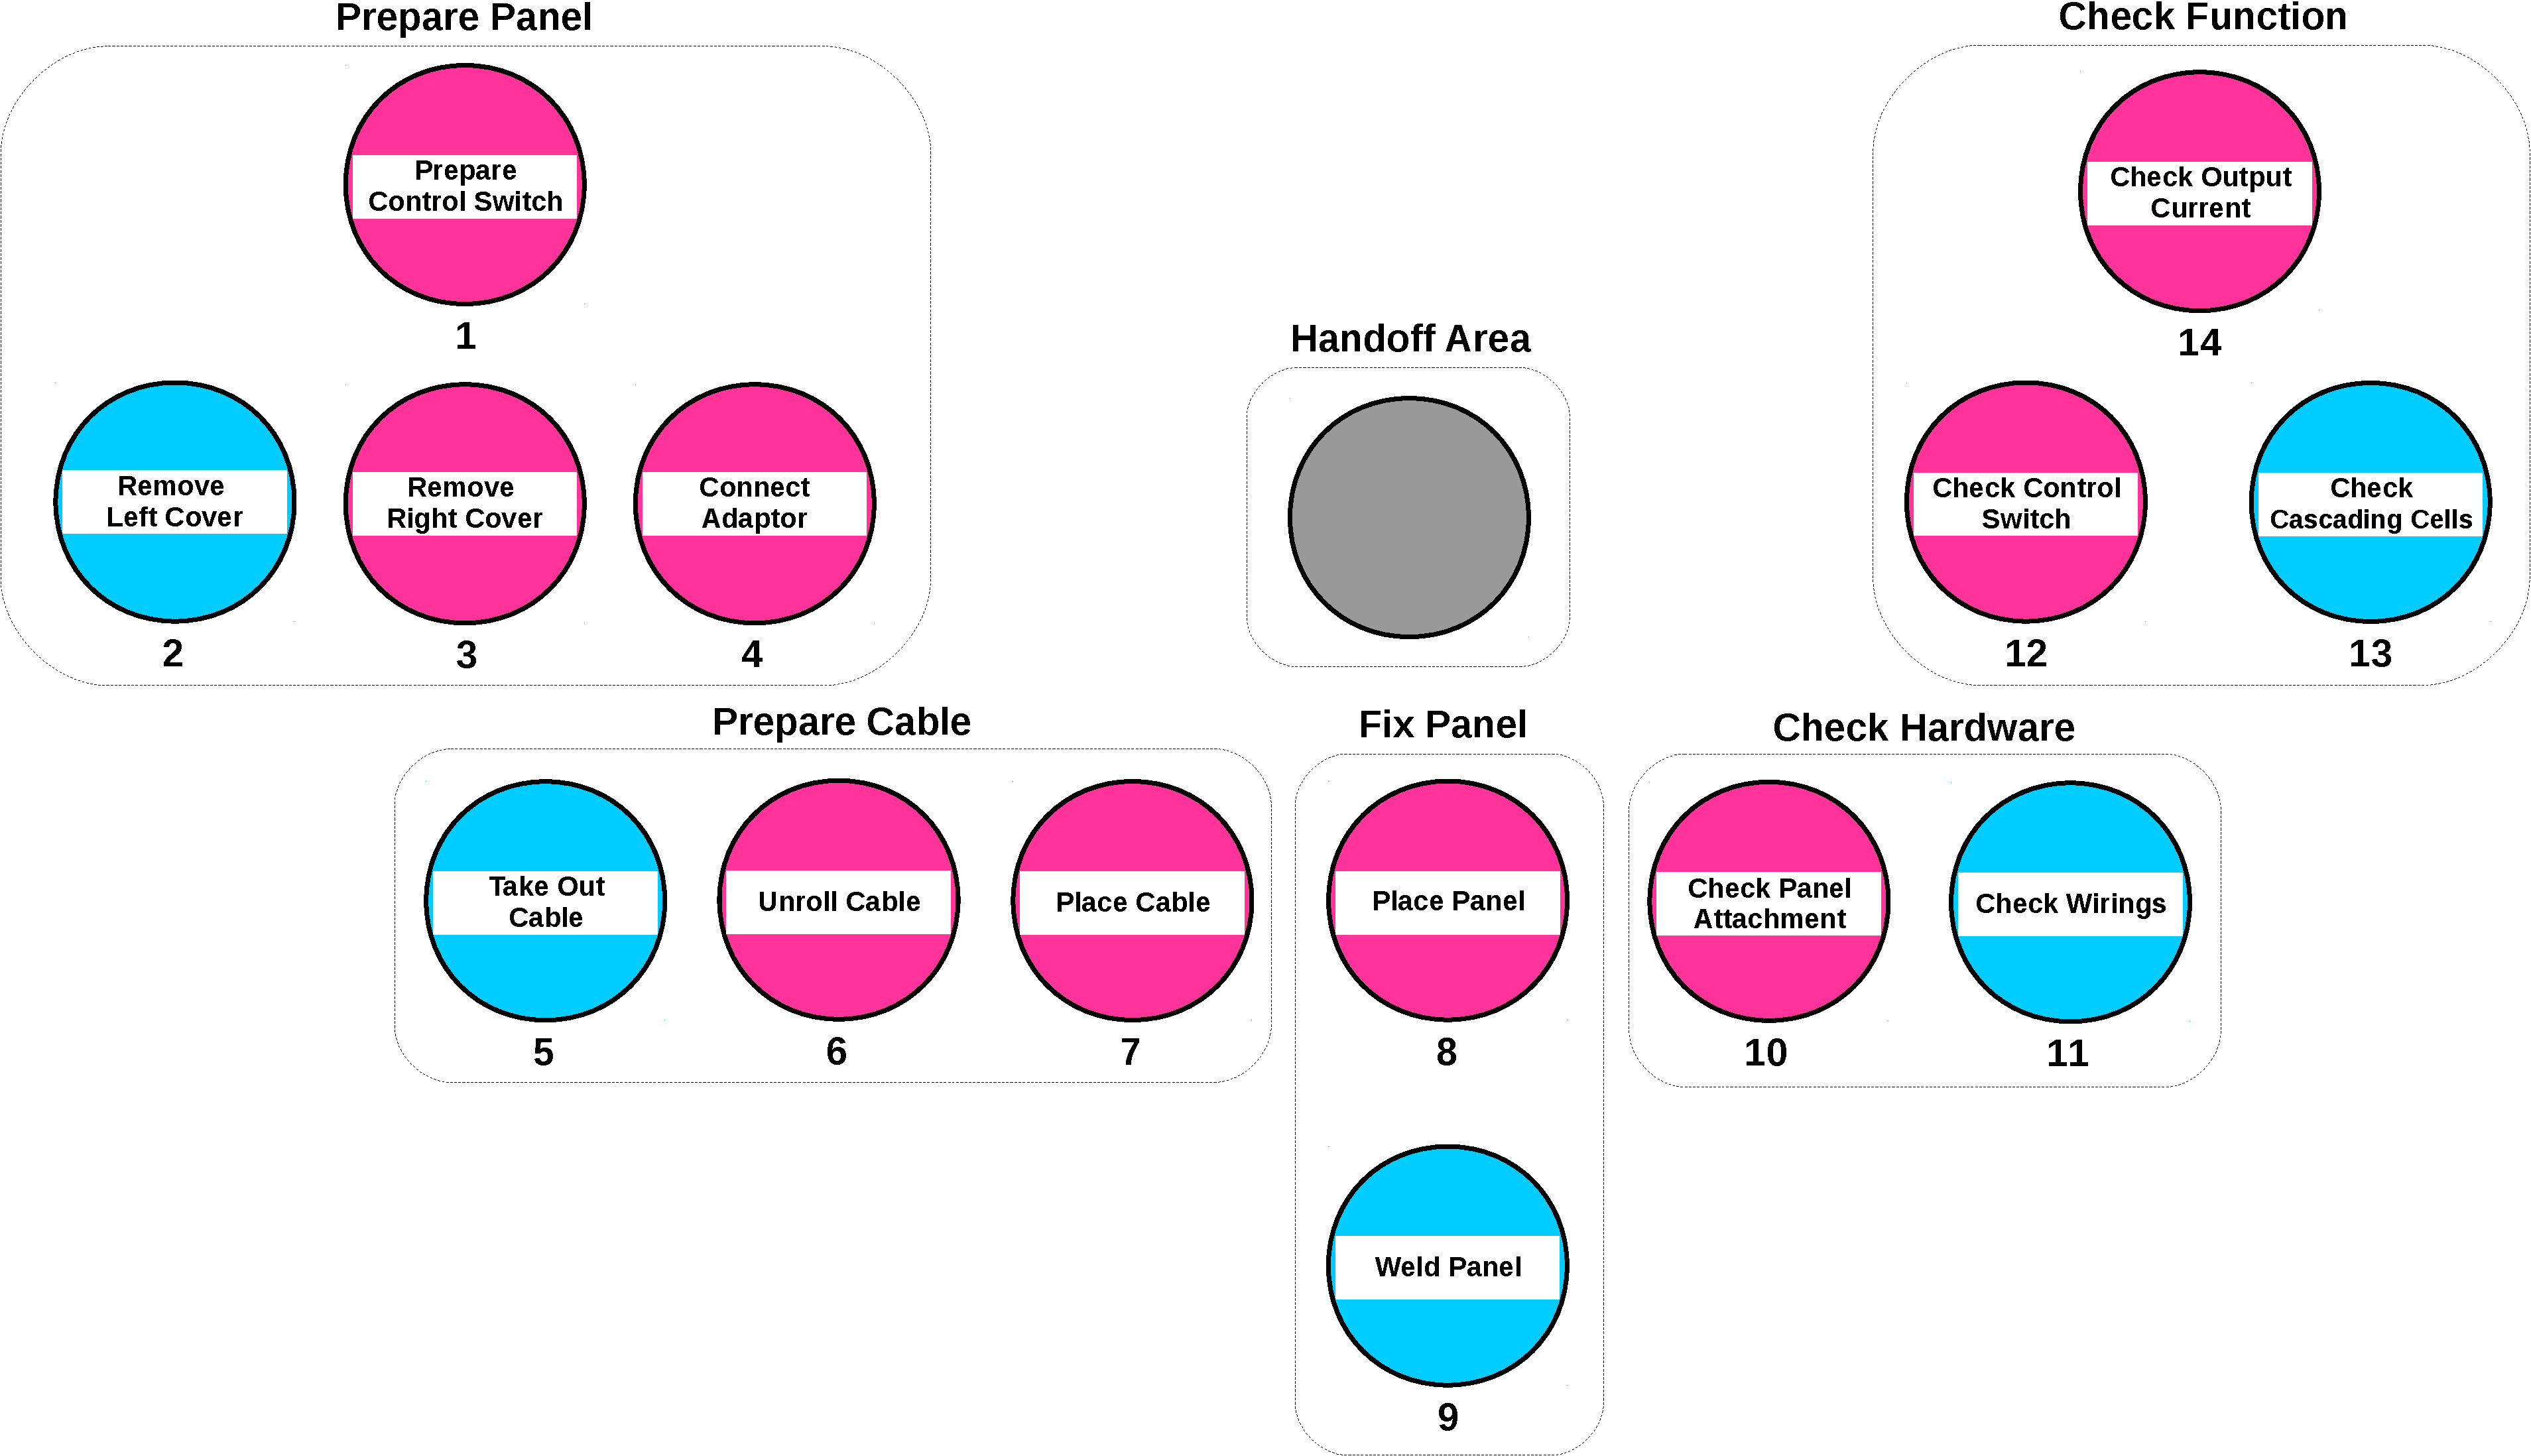
\includegraphics[width=0.48\textwidth]{figure/gameBoard.pdf}
  \caption{The layout of the available spots for the human and the robot to
  place their pegs during the collaboration.}
  \label{fig:game_board}
\end{figure}

\subsection{Environment and Tasks}

The environment was set up in Human-Robot Interaction lab. and included the
robot, the collaboration board on top of a desk, and the participant standing in
front of the robot on the other side of the board (see Figure
\ref{fig:environment}). One of the experimenters monitored the interactions
using a live stream of a camera in a different room. The experimenter provided
only the required perception, i.e., decision on success or failure of the tasks
for the robot, through the entire time of the collaboration (see Section
\ref{sec-interaction-paradigms}).

The tasks were defined based on the HTN structure shown in Figure XYZ and were
executed in a turn-taking fashion by either of the collaborators. For each task
either the robot or the participant was responsible to pick up one of the
corresponding pegs from their own inventory and place it on the right spot which
was colored and tagged same as the associated peg.

\begin{figure}
  \centering
  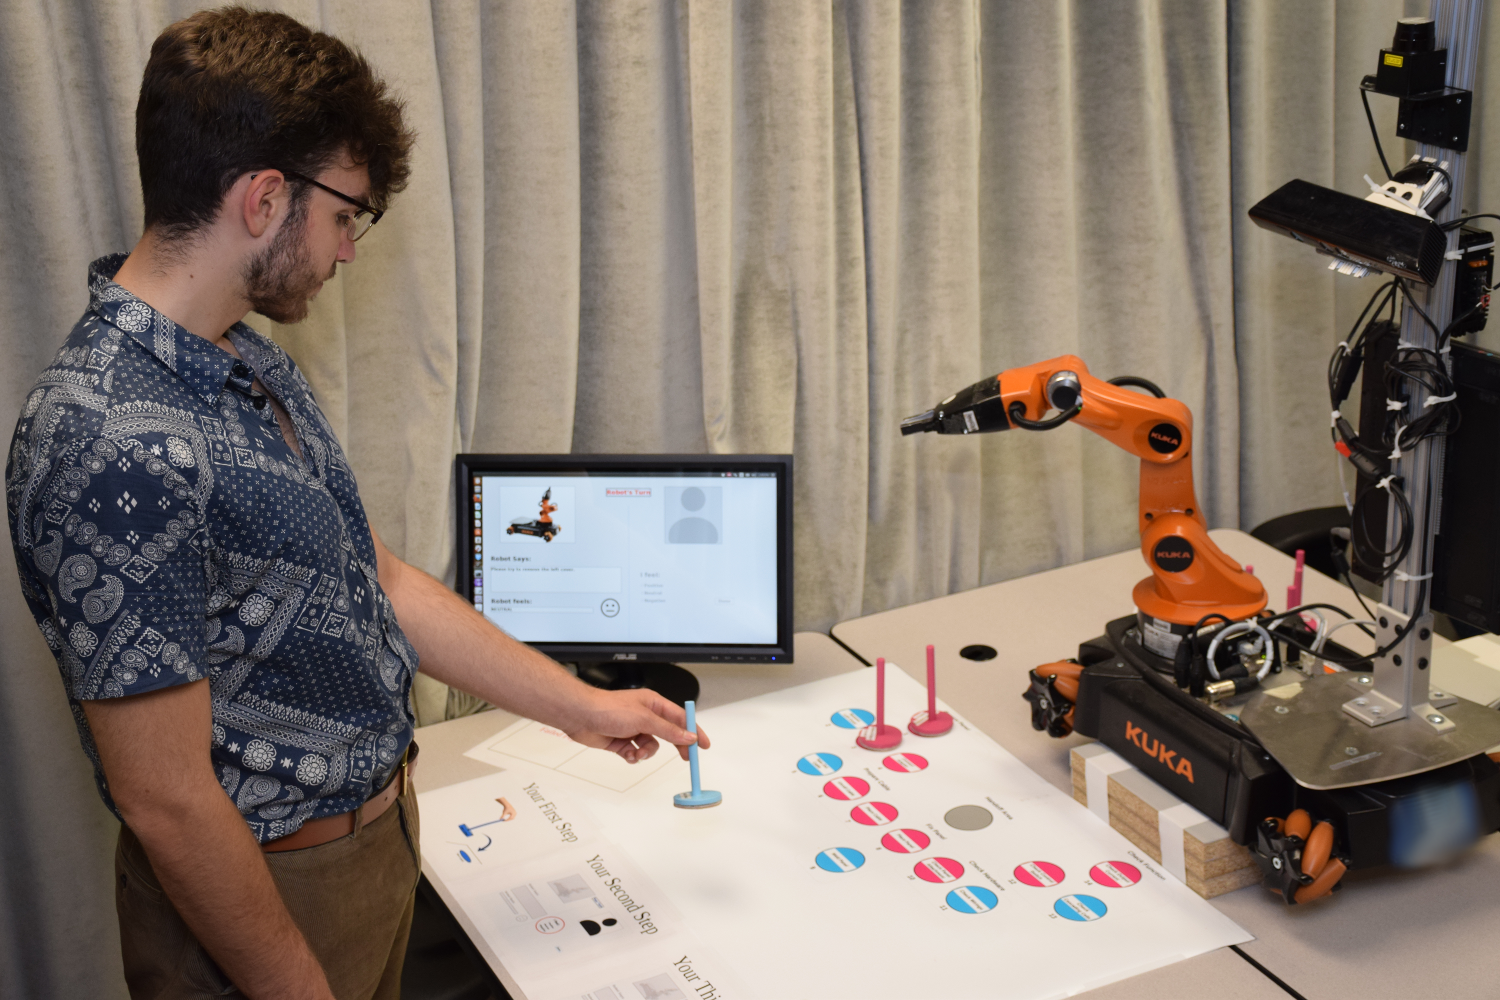
\includegraphics[width=0.45\textwidth]{figure/environment.png}
  \caption{{\fontsize{9}{9}\selectfont Experimental setup.}}
  \label{fig:environment}
\end{figure}

\section{Evaluation and Results}

\subsection{Hypothesis}

The non/social functions of emotions impact a collaboration process. Human
collaborators prefer to collaborate with others whose behaviors are influenced
by these functions of emotions depending on the context. We developed seven
hypotheses on positive influence of emotion-awareness and usefulness of emotion
function during collaboration:

\textit{\textbf{Hypothesis 1.}} Subjects will prefer to collaborate with the
robot which is controlled by Affective Motivational Collaboration framework more
than the robot which is controlled by Disco.

\textit{\textbf{Hypothesis 2.}} Subjects will find a mutual understanding in the
collaboration with the robot which is controlled by the AMC framework more than
the robot controlled by Disco.

\textit{\textbf{Hypothesis 3.}} Subjects will find working with the robot which
is controlled by AMC framework less confusing than the robot controlled by
Disco.

\textit{\textbf{Hypothesis 4.}} Subjects will find the robot which is controlled
by AMC framework understanding their goals more than the robot controlled by
Disco.

\textit{\textbf{Hypothesis 5.}} Subjects will find the robot which is controlled
by AMC framework understanding their feelings more than the robot controlled by
Disco.

\textit{\textbf{Hypothesis 6.}} Subjects will find the robot which is controlled
by AMC framework more helpful in compare to the robot controlled by Disco.

\textit{\textbf{Hypothesis 7.}} Subjects will find the robot which is controlled
by AMC framework more trustworthy than the robot controlled by Disco.

\subsection{Procedure}
Participants were first given a brief description of the purpose of the
experiment. After the short introduction, they were asked to review and sign a
consent form. Participants were then provided with a written instruction of
their task and the rules for collaborating with the robot. Then, one of the
experimenters lead them into the experiment room and asked the participants
to asked to answer pre-experiment questionnaires. Afterwards, the experimenter
went through all the important details of the instructions with the participants
standing in front of the collabortion board and the robot. The experimenter
confirmed participants' correct understanding of the tasks and informed them
with type of task failures that might occur during the collaboration.
Participants were told that researchers were developing a collaborative robot
and would like their help in evaluating their design. Participants were provided
with identical instructions and randomly assigned to the conditions in the
experiment. They were told that, after their collaboration with the robot, they
would be asked to answer a questionnaire on their experience. After completing
the first round of collaboration, participants answered a post-experiment
questionnaire that measured their perceptions of the robot, the task, and
the collaboration procedure. After answering the first post-experiment
questionnaire, participants were told that they were going to collaborate with
the robot one more time and the robot might not necessarily have the same
collaborative behavior. After completing the second round of collaboration,
participants were asked to answer the second post-experiment questionnaire which
included the same questions as the first post-experiment questionnaire. After
all, participants were asked to answer an open-ended questionnaire which
measured their perception of difference between two runs, their preference of
collaborative robot between two runs, and thier reasons of preference.

\subsection{Measurements}

In our study two basic conditions of the robot were tested: a) controlling the
robot using Disco, b) controlling the robot using AMC framework. The
collaborative results were measured using objective and subjective measurements.

\textit{\textbf{Objective -- }} We measured participants' recall of the
collaborative behaviors presented by the robot using an open-ended
post-experiment questionnaire. We also specifically asked the participants what
behavior of the robot did they like during their collaboration.

\textit{\textbf{Subjective -- }} We evaluated participants' levels of
satisfaction, trust, confusion, goal achievement, as well as mutual
understanding of goals, mutual understanding of feelings, mutual agreement, and
also participants' beliefs about the efficiency of collaboration and their
feeling of robot's collaborative behaviors. Seven-point Likert scales were used
in all questionnaire items.

\subsection{Participants}

A total of 37 participants participated in the experiment in 74 trials.
Participants were recruited from Worcester Polytechnic Institute's students and
staffs as well as other civilians recruited from outside of the campus. The ages
of the participants varied between 19 and 74 with an average of 34.2 years
before our screening of 4 subjects based on our sanity check questions. After
this screening the ages of the participants varied between 19 and 54 with an
average of 30.8 years old. Of all the 33 participants, 21 were female and 12
were male. Each participant participated in 2 trials. In one trial the robot was
controlled using Disco and in the second trial the robot was controlled using
AMC framework. The order of these two trials were randomly assigned to each
participant. In general we used Disco first in 16 experiments, and AMC framework
first in 17 experiments.

\begin{figure*}[tbh]
\centering
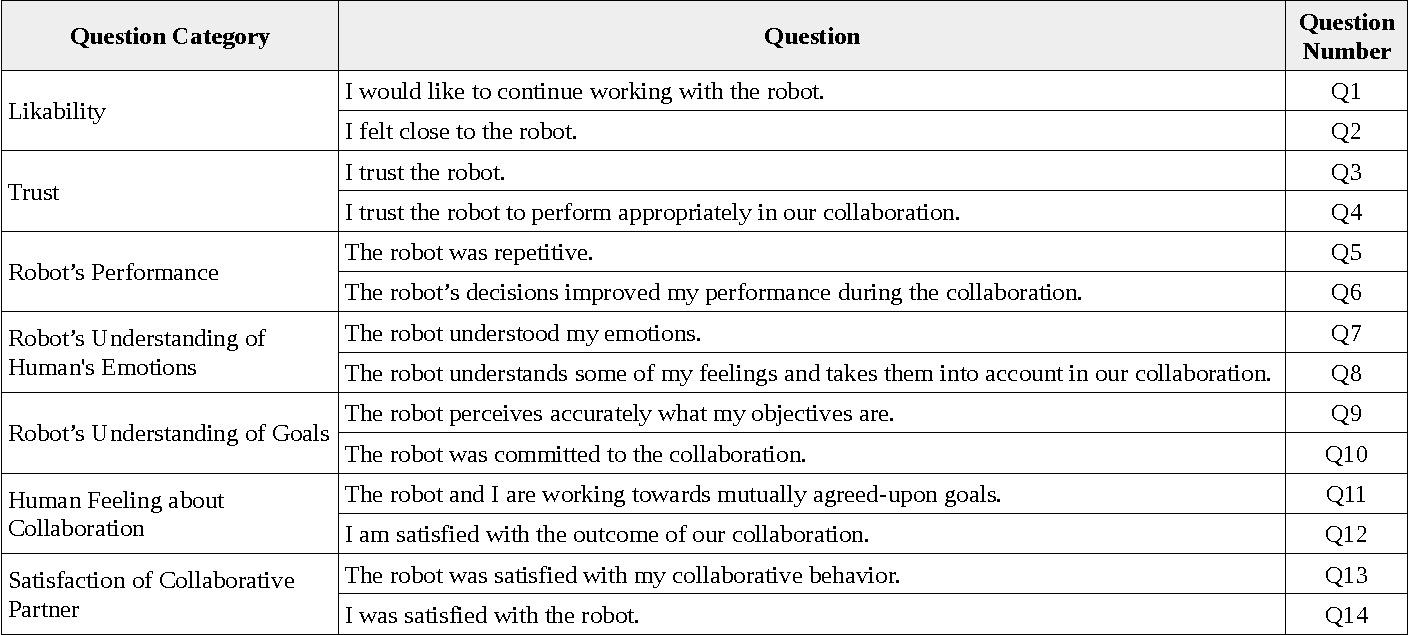
\includegraphics[width=0.98\textwidth]{figure/table1-croped.pdf}
\caption{A sample black and white graphic that has been resized with the
\texttt{includegraphics} command.}
\end{figure*}

\begin{figure*}[tbh]
\centering
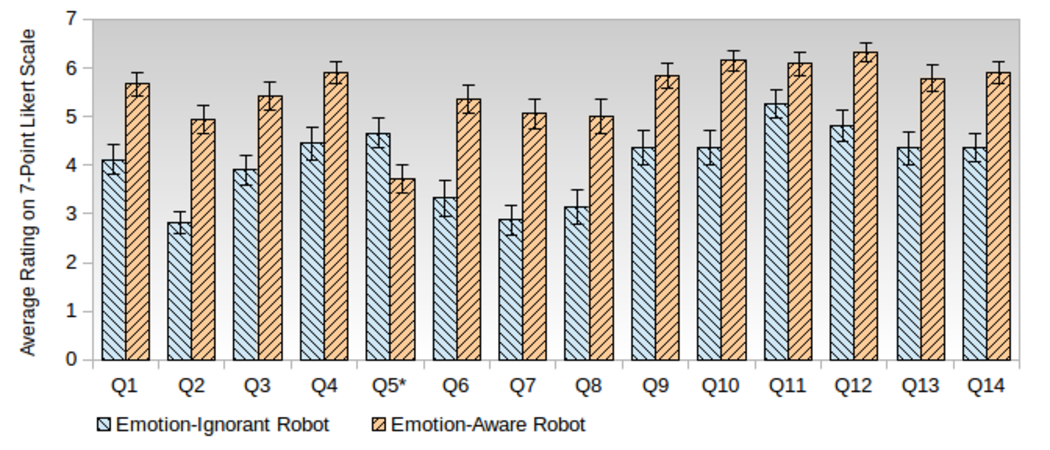
\includegraphics[width=0.9\textwidth]{figure/14Questions.pdf}
\caption{A sample black and white graphic
that has been resized with the \texttt{includegraphics} command.}
\end{figure*}

\begin{figure*}[tbh]
\centering
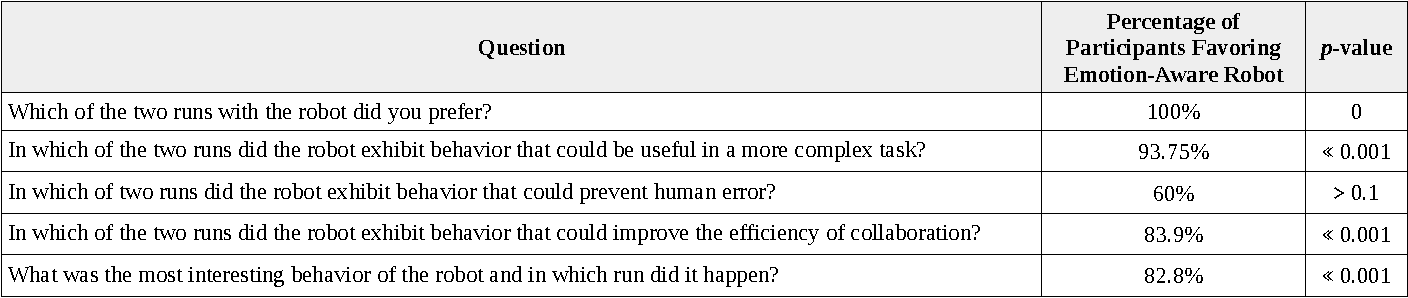
\includegraphics[width=0.98\textwidth]{figure/table2-croped.pdf}
\caption{A sample black and white graphic that has been resized with the
\texttt{includegraphics} command.}
\end{figure*}

\begin{figure*}[tbh]
\centering
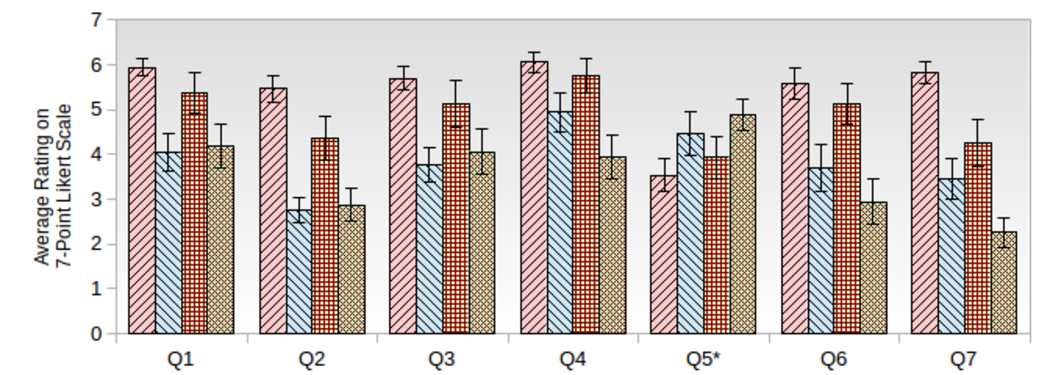
\includegraphics[width=0.9\textwidth]{figure/AgeComparison1.pdf}
\caption{A sample black and white graphic
that has been resized with the \texttt{includegraphics} command.}
\end{figure*}

\begin{figure*}[tbh]
\centering
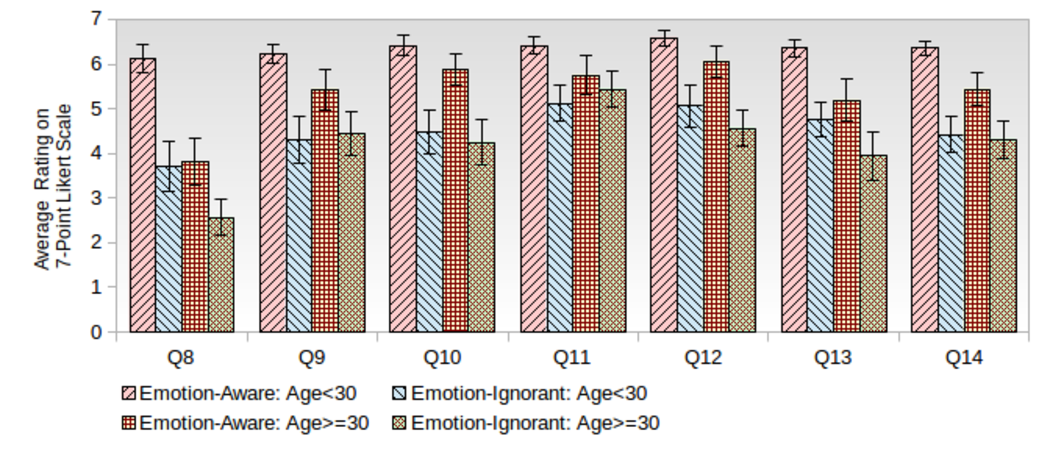
\includegraphics[width=0.9\textwidth]{figure/AgeComparison2.pdf}
\caption{A sample black and white graphic
that has been resized with the \texttt{includegraphics} command.}
\end{figure*}

\subsection{Evaluation Results}

\textit{\textbf{Subjective -- }} In our first hypothesis we predicted that the
participants would prefer to collaborate with the robot controlled by AMC
framework than the robot controlled by Disco. This prediction was supported by
our analysis. There was a significant difference across two conditions in
participants' preferrance to collaborate with the robot. In general ??? out of
33 participants preferred to collaborate with the robot controlled by AMC
framework; ??? out of 33 participants found at least one behvaior generated by
AMC framework useful for more complex tasks; ??? out of 33 participants found
the robot controlled by AMC framework being able to exhibit behaviors that can
prevent human errors; ??? out of 33 participants believe the robot controlled by
AMC framework can exhibit behaviors that could improve efficiency of
collaboration; and, ??? out of 33 participants mentioned at least one of the
collaborative behaviors of the robot controlled by AMC framework as an
interesting behavior during collaboration.

\textit{\textbf{Objective -- }} 

\section{Analysis and Discussion}

\subsection{Generalization and Limitations}

\section{Conclusions}


%ACKNOWLEDGMENTS are optional
\section{Acknowledgments}

%
% The following two commands are all you need in the
% initial runs of your .tex file to
% produce the bibliography for the citations in your paper.
\bibliographystyle{abbrv}
\bibliography{mshayganfar}  % sigproc.bib is the name of the Bibliography in
% this case You must have a proper ".bib" file
%  and remember to run:
% latex bibtex latex latex
% to resolve all references
%
% ACM needs 'a single self-contained file'!
%
%APPENDICES are optional
%\balancecolumns
\end{document}
